\section{Lecture 1}
\subsection{Lecture Notes - Lagrangian Mechanics Part 1}
\subsubsection{Newtonian Mechanics to Lagrangian Mechanics}
Recall the Newtonian formulation of classical mechanics; given the forces $\v{F}_1(t), \cdots \v{F}_n(t)$ on a particle, we can solve Newton's second law (a second order differential equation):
\[\sum_{i=1}^n \v{F}_i(t) = m \ddot{\v{r}}(t)\]
To obtain the trajectory $\v{r}(t)$, which is uniquely determined by the initial conditions $\v{r}(t_0)$ and $\dot{\v{r}}(t_0)$. 

In this course, we will begin by looking at the Lagrangian formulation of classical mechanics. While this formulation contains no new physics compared to the Newtonian formulation, there are two distinct benefits:
\begin{enumerate}
    \item We can obtain EOM that do not depend on the coordinate system
    \item It is easier to treat constrained systems. 
\end{enumerate}
\subsubsection{The Variational Principle Setup}
To do this, we will use a new approach, known as the \textbf{Variational principle}. To set this up, let us consider the trajectory (as well as some "wrong" paths between the same two endpoints) travelled by a particle:
\begin{center}
    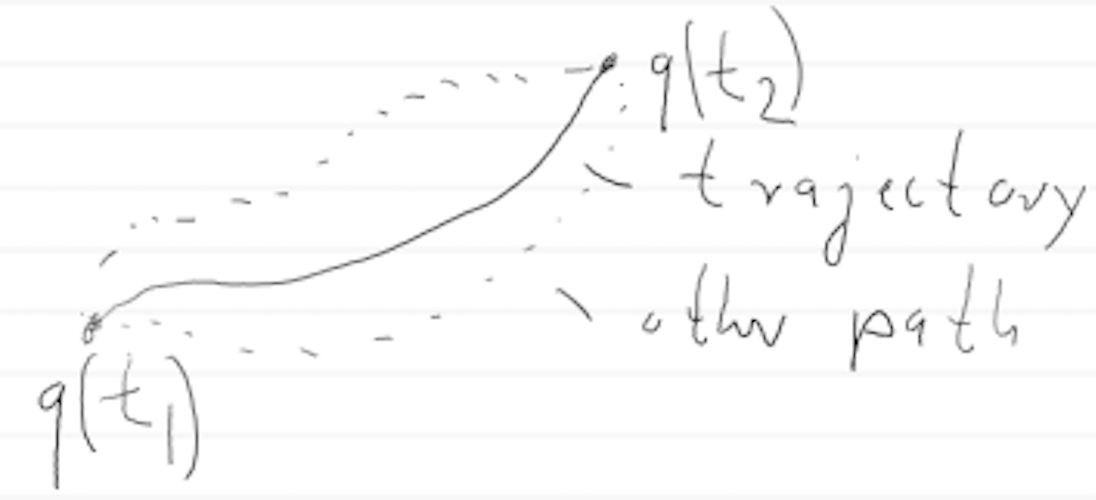
\includegraphics[scale=0.4]{Lecture-1/L1-img1.png}
\end{center}
The trajectory from time $t_1$ to $t_2$ is parametrized by the generalized coordinate $q$. Examples of these are $x_1, y_1, \theta_1$. 
\subsubsection{Generalized Coordinates}
For $N$ particles, a generalized coordinate $q_i$ depends on the positions of the $N$ particles:
\[q_i = q_i(\v{r}_1, \cdots, \v{r}_N)\]
In Cartesian coordinates, we have $3N$ coordinates but these are not necessarily independent. In general, we may have constraint functions $f_\alpha(\v{r}, \dot{\v{r}}, t) = 0$ where $\alpha = 1, \cdots, k$ (i.e. $k$ constraints). We then have $q_i$ independent coordinates, where $i = 1, \cdots n$ where $i = 3N - k$. In other words, for a system of $N$ particles, we have $3N - k$ independent/generalized coordinates. Generalized coordinates allow us to avoid worrying about the constrained parameters. 
\subsubsection{Hamilton's Principle and the Lagrangian}
Let us consider assigning to each generalized coordinate $q(t)$ a number/value:
\[q(t) \mapsto S[q(t)] \in \RR\]
This is a functional (as denoted by the square brackets), as it takes in a function as an argument. Now, let us consider \textbf{Hamilton's principle}:
\begin{center}
    \textit{The actual path of a particle between times $t_1$ and $t_2$ is such that the line integral:
    \[ S[q] = \int_{t_1}^{t_2} \LL(q_1, \dot{q}_1, t) dt\]
    is stationary.}
\end{center}
Though the principle saysthe integral is stationary, often this correponds to a minimum (though not always). The function $\LL$ is defined as:
\[\LL = T - U\]
where $T$ is the kinetic energy and $U$ is the potential energy. This is called the \textbf{Lagrange Function} or \textbf{Lagrangian}. $S$ is called the \textbf{action}. Though we have not shown it explicitly, this Lagrange function gives the correct trajectory. Note that we have in essence replaced a second order ODE (Newton's second law) with an integral of $\LL$. Having two endpoints $t_1$ and $t_2$ is consistent with the two initial conditions for a second order ODE. 